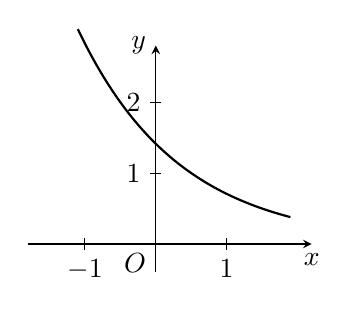
\begin{tikzpicture}[>=stealth, scale=0.9]
  % 坐标轴
  \draw[->] (-1.8, 0) -- (2.2, 0) node[below] {$x$};
  \draw[->] (0, -0.4) -- (0, 2.8) node[left] {$y$};
  \node[below left] at (0, 0) {$O$};

  % 刻度
  \draw (-1, 0.08) -- (-1, -0.08) node[below] {$-1$};
  \draw (1, 0.08) -- (1, -0.08) node[below] {$1$};
  \draw (0.08, 1) -- (-0.08, 1) node[left] {$1$};
  \draw (0.08, 2) -- (-0.08, 2) node[left] {$2$};

  % 指数函数曲线 (例如 a=0.5, b=0.5 即 y = 0.5^(x - 0.5))
  \draw[thick, domain=-1.1:1.9, samples=50] plot (\x, {pow(0.5, \x - 0.5)});
\end{tikzpicture}
